\documentclass[twocolumn]{article}

\usepackage[utf8]{inputenc}
\usepackage[T1]{fontenc}
\usepackage{amsmath}
\usepackage{amsthm}
\usepackage{amsfonts}
\usepackage{graphicx}
\usepackage{breqn}

\newtheorem{lemma}{Lemma}
\newtheorem{theorem}{Theorem}

\newcommand{\beq}{\begin{eqnarray}}
\newcommand{\eeq}{\end{eqnarray}}

\DeclareMathOperator{\wbf}{wBF}

\title{DRAFT: Scalable, Robust Multipath Communication on the Butterfly Network}
\author{
    Edward L. Platt\\
    elplatt@umich.edu
    \and
    Daniel M. Romero\\
    drom@umich.edu
}
\date{January 2016}

\begin{document}

\maketitle

\section{Introduction}

\section{Trust Model}

We assume that a sender $A$ (or Alice) wants to send sensitive information
to a receiver $B$ (or Bob).
Alice and Bob are both nodes on a communication network represented by a graph
$G = (V, E)$.
Two nodes are connected when they are able to communicate directly with each
other.
We also assume the presence of an adversary $C$ (or Eve) who wishes to disrupt
that communication by altering or delaying the transmission.
Eve has compromised a subset of nodes and has full control over their behavior.
Any transmission routed through a compromised node is considered faulty.
Alice and Bob do not know which nodes have been compromised.

In our model, links also represent trust.
Specifically, two nodes are connected if each node believes that the other
has not been compromised by its adversary.
In other words, a communication link is severed if one node believes the other
to be compromised.
If trust were transitive, a connected path from Alice to Bob, would guarantee
a trusted channel, but trust is not transitive \cite{christianson_why_1997}.
Rather than entirely abandoning transisitivy, we assume that trust is
partially transitive.
Specifically each node has a {\em trusted neighborhood} of nodes up to $h$ hops
away, which we assume have not been compromised by that node's adversaries.
Our objective is now to construct a robust communication channel from Alice's
trusted neighborhood to Bob's.

\section{Multipath Fault Tolerance}

We achieve robust communication between trusted neighborhoods through
Concurrent Multipath Routing (CMR) \cite{}.
If there are multiple {\em redundant paths} (i.e., paths sharing no nodes or
links) between Alice and Bob's trusted neighborhoods, multiple copies of a
message can be sent along different paths, enabling standard error detection and
error correction techniques to be applied at the destination.
If Alice randomly selects $k$ of $n$ total redundant paths, Eve's best strategy
is to compromise at least one node on as many of the paths as possible.
Because an error can be detected if even a single copy has been tampered with,
Eve must compromise all $k$ paths in order to convince Bob to accept a compromised
message.
If Eve has the resources to compromise $l$ total nodes, the probability that
Bob receives an undetectable error is:
\beq
\label{eq:pe}
p_e &=& \frac{l!(n-k)!}{n!(l-k)!}.
\eeq
Letting $k=\alpha n$ and $l=\beta n$, then applying Stirling's
approximation gives:
\begin{eqnarray}
\nonumber
p_e &\approx&
\frac{\sqrt{\beta(1-\alpha)}}{\sqrt{\beta-\alpha}} \\
& &
\times {}
\label{eq:pe_approx}
\left[
    \left( \frac{\beta-\alpha}{1-\alpha} \right)^{\alpha}
    \left( \frac{\beta}{\beta-\alpha} \right)^{\beta}
    (1-\alpha)
\right]^n
\end{eqnarray}
Note that Eq. (\ref{eq:pe_approx}) is exponential in the number of redundant
paths $n$, which depends only on the network structure, and not on the
resources available to individual nodes.
If a network has a large number of redundant paths between trusted neighborhoods,
a very low probability of undetected errors can be achieved, even if an adversary
has the resources to compromise a very large fraction of the avialable paths.
The value of $p_e$ for various $k$, $l$, and $n$ is shown in Figure
\ref{fig:perror}.

\begin{figure}
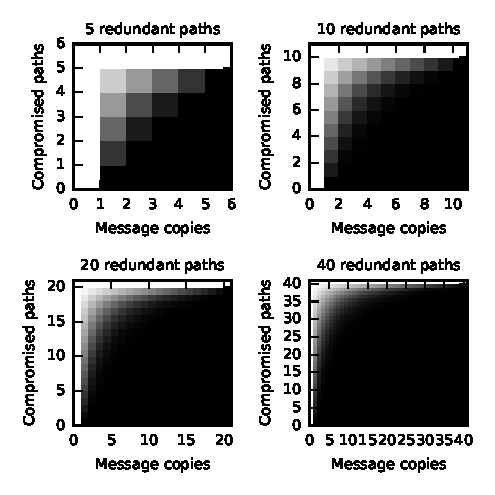
\includegraphics{fig-perror.pdf}
\caption{
Probability $p_e$ of an undetected error as a function of the number of message
copies $k$ and compromised paths $l$.
\label{fig:perror}
}
\end{figure}

\section{Butterfly Network}

We now describe a Concurrent Multipath Routing scheme on a specific family
of networks: the butterfly network \cite{}.
Several variations on the butterfly network exist.
Specifically, we utilize the wrap-around butterfly.
We define the $m$-dimensional directed wrap-around butterfly $\wbf(m)$:
\beq
\wbf(m) &=& (V, E_\downarrow \cup E_\rightarrow) \\
V &=& \mathbb{Z}_m \times \mathbb{Z}_{2^m} \\
E_\downarrow &=& \{((l,z),(l+1 (\text{mod } m),z) \nonumber \\
&& \; | \, l \in \mathbb{Z}_d, z \in \mathbb{Z}_{2^m}\} \\
E_\rightarrow &=& \{(l,z),(l+1 (\text{mod } m), z \oplus 2^l) \nonumber \\
&& \; | \, l \in \mathbb{Z}_d, z \in \mathbb{Z}_{2^m}\},
\eeq
where $\oplus$ represents the bitwise XOR operator.
Each node is associated with a level $l$ and an $m$-bit integer $z$.
There are two types of edges, shown in Figure \ref{fig:butterfly}.
Down edges ($E_\downarrow$) connect nodes sharing the same $z$ value
in a cycle of increasing level $l$.
Down-right edges ($E_\rightarrow$) also link to a node of level $l + 1$,
but one having the bitstring equal to $z$ with the $l$th bit flipped.

The wrap-around butterfly network has a number of properties making it useful for multipath routing:
\begin{description}
\item[Vertex transitivity]
The problem
of finding a route between arbitrary nodes $v$ and $w$
can be reduced to finding a route from node $(0,0)$ to some $\tilde{w}$.
\item[Logarithmic diameter]
For any two nodes, the length of the shortest path between them is logorithmic
in the size of the network.
\item[Constant degree]
In practical applications, each communication link requires additional resources,
such as physical infrastructure or entries in a routing table.
A constant degree limits the number of such resources needed as the network
grows in size.
\end{description}

\begin{figure}
\begin{center}
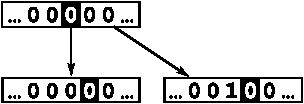
\includegraphics{fig-butterfly.pdf}
\end{center}
\caption{
Schematic illustration of the two types of edges in a directed butterfly network.
The node $(l,z)$ is shown as the bit string $z$ with a square around the $l$th bit.
\label{fig:butterfly}
}
\end{figure}

\subsection{Multipath Routing on the Butterfly Network}

We now describe a routing scheme that provides $2^h$ redundant paths between
the $h$-hop trusted neighborhoods of any two nodes in an $m$-bit
wrap-around butterfly network.
Utilizing vertex transitivity, we label the source node as $(0, 0)$ and
denote the destination node as $w = (l_w, z_w)$.

Let $s$ be an integer such that $0 \leq s < 2^h$.
Let $v_s^{(t)} = (l^{(t)}, z^{(t)})$ be the $t$th node in the path labeled by $s$.
For convenience, we will omit the subscript $s$.
We define two partitionings of the integers in $\mathbb{Z}_{2^m}$:
one having the lowest $h$ bits matching the
bits of $s$, and one having the $h$ bits preceeding the destination level $l_w$
matching $s$:
\beq
S_s &=& \{z \in \mathbb{Z}_{2^m} | \forall i \in \mathbb{Z}_h z_i = s_i \} \\
R_s &=& \{z \in \mathbb{Z}_{2^m} | \forall i \in \mathbb{Z}_h z_{(l_w - h + i)} = s_i \}.
\eeq
Note that if $r \neq s$, then $S_s \cap S_r = R_s \cap R_r = \emptyset$.

We now construct a path such that between trusted neighborhoods $z^{(t)}$ is always
in $S_s$, $R_s$, or both, guaranteeing that the path does not overlap with the
other paths $v_r^{(t)}$.
Routing proceeds in stages, with the level $l$ increasing by 1 at each hop.
In Stage 1 ($0 \leq t < h$), down or down-right edges
are chosen such that the the $t$th bit of $z^{(t+1)}$ is equal to the $t$th bit
of $s$. Throughout Stage 1, all nodes are within the sender's trusted neighborhood.
At the end of Stage 1, $z^{(h)} \in S_s$, and $z^{(t)}$ will remain so until the level loops
back to $0$ at $t = m$.

In Stage 2 ($h \leq t < l_w - h$), edges are chosen to make the $t$th bit of
$z^{(t+1)}$ match the $t$th bit of $z_w$.

In Stage 3 ($l_w - h \leq t < l_w$), the bits of $z^{(t)}$ are chosen to match $s$,
such that after the stage is complete, $z^{(l_w)} \in R_s$.

In Stage 4 ($l_w \leq t < m$), as in stage 2,
paths are chosen such that the $t$th bit of $z^{(t+1)}$ matches $z_w$.
After Stage 4, all bits of $z^{(m)}$ are equal to those of $z_w$
except for the first $h$ and the $h$ preceeding index $l_w$.
$z^{(m)}$ is also in both $S_s$ and $R_s$.

At this point, we define $\tau = t - m$.
In Stage 5 ($0 \leq \tau < h$), the first $h$ bits of $z^{(t)}$ are set to
match $z_w$, potentially removing $z^{(t)}$ from $S_s$.

In Stage 6 ($h \leq \tau < l_w - h$), all down edges are chosen, incrementing
the level without any effect on $z^{(t)}$.
At the end of Stage 6, $z^{(m + l_w - h)}$ is still in $R_s$ and
$v^{(m + l_w - h)}$ is now within the trusted neighborhood of $w$.

In the seventh, and final stage ($l_w - h \leq \tau < l_w$), the $h$ bits of $z^{(t)}$
preceeding index $l_w$ are set to match $z_w$.
After this stage, $v^{(m + l_w)} = w$ and routing is complete.

\begin{figure}
\begin{center}
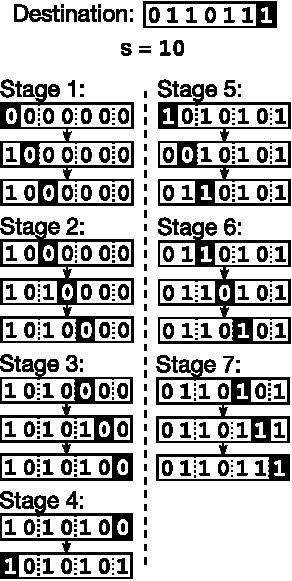
\includegraphics{fig-routing.pdf}
\end{center}
\caption{
\label{fig:routing}
}
\end{figure}

\section{Discussion}

\section{Conclusion}

\bibliographystyle{plain}
\bibliography{netft}

\end{document}
